% This is samplepaper.tex, a sample chapter demonstrating the
% LLNCS macro package for Springer Computer Science proceedings;
% Version 2.20 of 2017/10/04
%
\documentclass[runningheads]{llncs}
%
\usepackage{graphicx}
\usepackage{url}
\usepackage{subfigure}
\usepackage{subcaption}
\usepackage{float}
\usepackage{subfloat}
\usepackage{caption}

\begin{document}
%
\title{ATP Tennis Player Network Analysis}

\author{Kuang-Yu Li}

\institute{INFOTECH, University of Stuttgart
\email{st169971@stud.uni-stuttgart.de}}
%
\maketitle              % typeset the header of the contribution
%
\begin{abstract}
In this project, an ATP(Association of Tennis Professionals) player network 
based on tennis match statistics of ATPWorld Tour was built and analyzed.
The goal for this project is to discuss the correlation of several centrality rankings with 
real-world qualities of players. In the end, I landed on a conclusion that Kat centrality is the most
suitable centrality. Top 10 ranking of Kat centrality is almost aligned with the real-world evaluation of 
player. Moreover, with the comparison for different network models, the player network exhibits the 
property of scale-free network. 

\keywords{Network  \and Katz centrality \and Scale-free.}
\end{abstract}
%
%
%
\section{Introduction}
I picked this topic not only because I am big tennis fan but also because I interested in evaluating evaluating players from the match result for the past 20 years. 
ATP stands for Association of Tennis Professionals, which is male professional tennis. ATP currently has over 1800 active players. ATP holds over 60 tennis tournaments with over 2000 matches worldwide. These tournaments are categorized into several categories according to its "points". 
Fig.~\ref{fig_example} gives an example of the point that winner can score in each tournament. Almost all tournaments are held in a single-elimination fashion. This means a player is dropped out from the tournament once he loses a match. The draw of the tournament is based on ATP ranking to separate top-ranked players from encountering each other in the early stage of tournament. With single elimination and rank-based draw, a "lucky" champion can not happen.
As mentioned above, ATP has its ranking, called ATP ranking. This ranking is also know as "world ranking". The ranking is a 52-week rolling ranking and is updated on a weekly basis. The rules of ATP ranking is only for active player. There are other ranking which focus on different aspect of player performance, such as Grand Slams ranking and GOAT points ranking. All of these rankings has its limitation.ATP ranking system only includes  active players. It is not logical to compare the retired players with active ones simply based on their rankings since they may not in the same period. For example, both Roger Federer and Andre Agassi were ranked no.1 in ATP during their prime years. I hope that by constructing a network from match statistic I could gain further insights in player evaluation. 

\todo[1] {add more comments}
Real data is collected from ATP match statistic from 1996~2016. A network is constructed based on this graph. 
Each node represent a tennis player. An edge represents a match fought between two players. Each each has an attribute of "weight", indicating the total number of matches.
To simplify the analysis of network, I chose my network to be a undirected graph with weighted edge.
After constructing the network, there are 3,035 nodes and 45,563 edges

Fig.~\ref{fig_0_simple_example} gives a zoomed in part of my tennis player network.
Fig.~\ref{fig_mynk} shows the complete graph of my network.


For citations of references, we prefer the use of square brackets
and consecutive numbers. The following bibliography provides
a sample reference list with entries for journal
articles~\cite{ref_article1}, a book~\cite{ref_book1}, proceedings without editors~\cite{ref_proc1},
and a homepage~\cite{ref_url1}. Multiple citations are grouped
\cite{ref_article1,ref_book1},
\cite{ref_article1,ref_book1,ref_proc1,ref_url1}.


\begin{figure}
\includegraphics[width=\textwidth]{0_simple_example}
\caption{A figure caption is always placed below the illustration.
Please note that short captions are centered, while long ones are
justified by the macro package automatically.} \label{fig_0_simple_example}
\end{figure}

\begin{figure}
\includegraphics[width=\textwidth]{1_graph}
\caption{A figure caption is always placed below the illustration.
Please note that short captions are centered, while long ones are
justified by the macro package automatically.} \label{fig_mynk}
\end{figure}


\section{Structural Insight}
Here goes all the analysis of your network. Fig.~\ref{fig_2_Degree_dist_hist} gives an example of a figure.


% Figure for Network Analysis Section

\begin{figure}
    \centering
    \begin{minipage}{0.5\textwidth}
        \centering
        \includegraphics[width=\textwidth]{2_Degree_dist_hist} % first figure itself
        \caption{Degree dist. Histogram}
        \label{fig_2_Degree_dist_hist}
    \end{minipage}\hfill
    \begin{minipage}{0.5\textwidth}
        \centering
        \includegraphics[width=\textwidth]{2_Degree_dist_log} % second figure itself
        \caption{Degree dist. logscale}
        \label{fig_2_Degree_dist_log}
    \end{minipage}
\end{figure}

\begin{figure}
    \centering
    \begin{minipage}{0.5\textwidth}
        \centering
        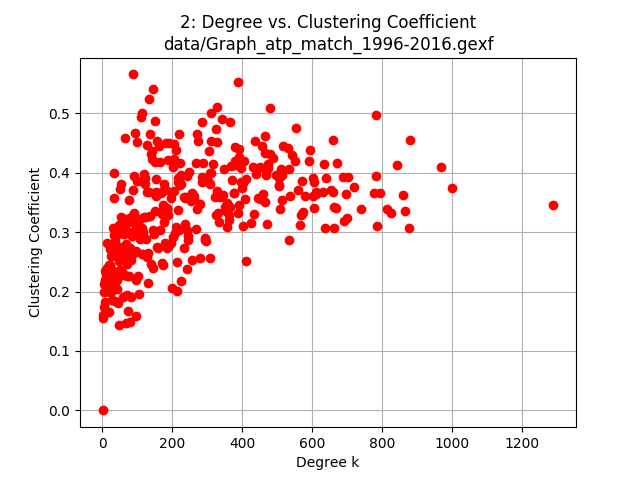
\includegraphics[width=\textwidth]{2_clustering_coeff} % first figure itself
        \caption{Clustering Coeff}
        \label{fig_2_clustering_coeff}
    \end{minipage}\hfill
    \begin{minipage}{0.5\textwidth}
        \centering
        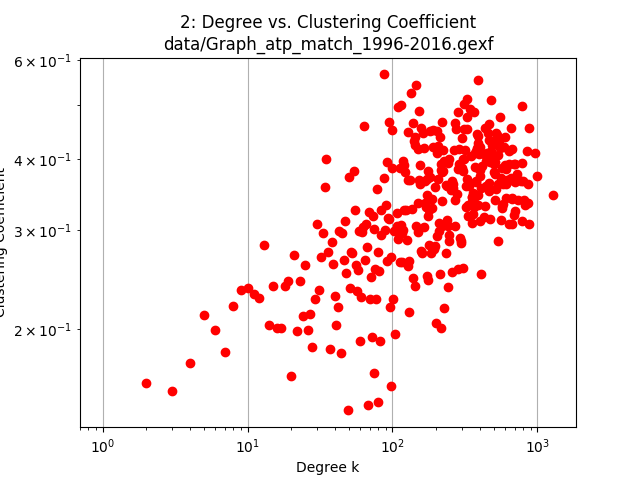
\includegraphics[width=\textwidth]{2_clustering_coeff_log} % second figure itself
        \caption{Clustering Coeff logscale}
        \label{fig_2_clustering_coeff_log}
    \end{minipage}
\end{figure}


\begin{figure}
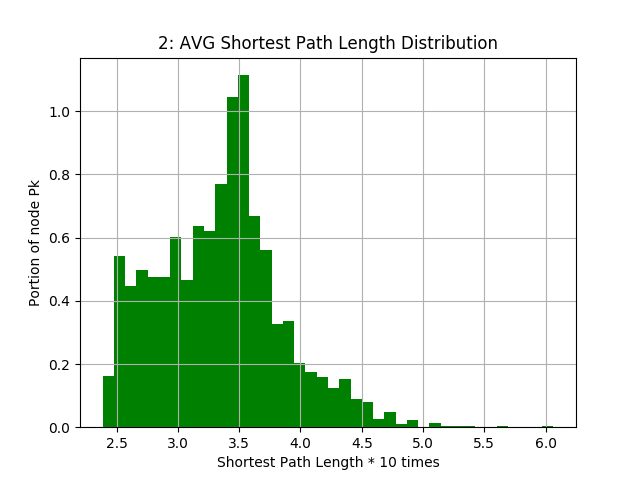
\includegraphics[width=\textwidth]{2_distance_distribution_hist}
\caption{Distance Distribution} \label{fig_2_distance_distribution_hist}
\end{figure}


\begin{figure}
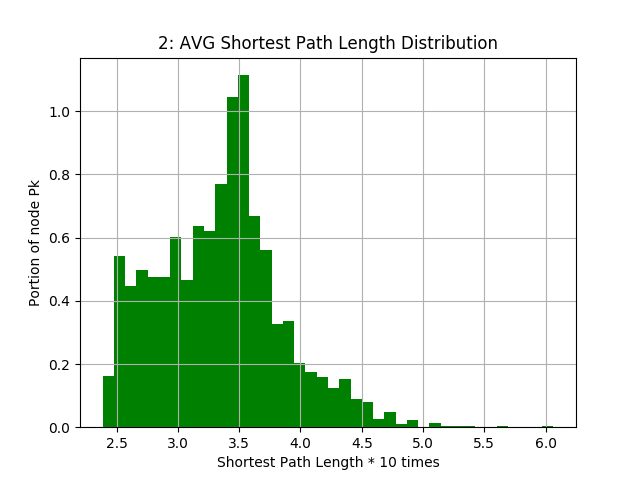
\includegraphics[width=\textwidth]{2_distance_distribution_hist}
\caption{Distance Distribution} \label{fig_2_distance_distribution_hist}
\end{figure}


\begin{figure}
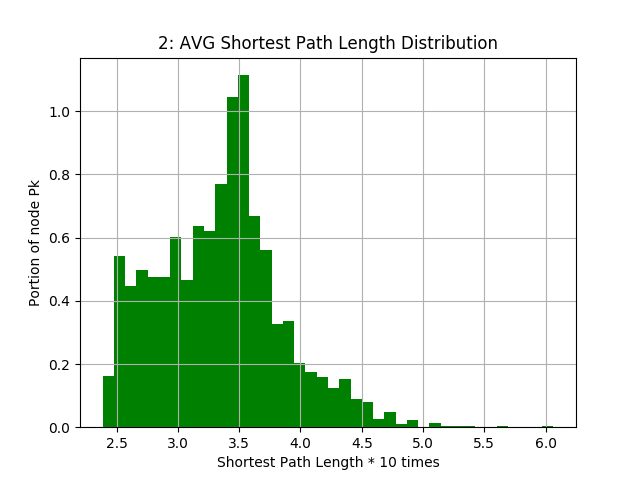
\includegraphics[width=\textwidth]{2_distance_distribution_hist}
\caption{Distance Distribution} \label{fig_2_distance_distribution_hist}
\end{figure}

\begin{figure}
\includegraphics[width=\textwidth]{2_ego_FEDERER}
\caption{Federer Ego Network} \label{fig_22_ego_FEDERER}
\end{figure}


\begin{figure}
    \centering
    \begin{minipage}{0.5\textwidth}
        \centering
        \includegraphics[width=\textwidth]{2_k_core_my} % first figure itself
        \caption{78-Core Graph}
        \label{fig_2_k_core_my}
    \end{minipage}\hfill
    \begin{minipage}{0.5\textwidth}
        \centering
        \includegraphics[width=\textwidth]{2_max_clique} % second figure itself
        \caption{Maximal Clique}
        \label{fig_2_max_clique}
    \end{minipage}
\end{figure}


Table~\ref{tab_my} an example of a table.
\todo{make table in the center}

Table~\ref{tab_ego} an example of a table.

% Table for Structural Insight Section
\begin{table}
\caption{Structural Metrics of my network.}\label{tab_my}
\begin{tabular}{|l|l|}
\hline
metric & value \\
\hline
order & 3,035 \\
size & 45,563 \\
density & 0.009896 \\
diameter & 8 \\
radius & 4 \\
average path length & 3.263307 \\
average clustering coefficient & 0.004897 \\
transitivity & 0.350256 \\
number of triangle & 745,720 \\ 
number of clique & 12,066,625 \\
number of component & 1\\
\hline
\end{tabular}
\end{table}




\begin{table}
\caption{Structural Metrics of ego network.}\label{tab_ego}
\begin{tabular}{|l|l|}
\hline
metric & value \\
\hline
order & 303 \\
size & 16,047 \\
density & 0.350731 \\
diameter & 2 \\
radius & 1 \\
average path length & 1.649269 \\ 
average clustering coefficient & 0.028295 \\ 
transitivity & 0.589713 \\ 
number of triangle & 404,647 \\ 
number of clique & 5,621,903 \\ 
number of component & 1 \\ 
\hline
\end{tabular}
\end{table}

Table~\ref{tab_kcore} an example of a table.
\begin{table}
\caption{Structural Metrics of k-core network.}\label{tab_kcore}
\begin{tabular}{|l|l|}
\hline
metric & value \\
\hline
order & 162 \\
size & 8954 \\
density & 0.686604 \\
diameter & 2 \\
radius & 2 \\
average path length & 1.313396 \\
average clustering coefficient & 0.039433 \\
transitivity & 0.744889 \\
number of triangle & 252,986 \\
number of clique & 6,800,942 \\
number of component & 1 \\
\hline
\end{tabular}
\end{table}






\section{Centrality Insight}

Table~\ref{tab_h_vs_b} an example of a table.
Table~\ref{tab_degree_vs_eigen} an example of a table.
Table~\ref{tab_katz_vs_page} an example of a table.

\begin{table}
\centering
\caption{Harmonic vs. Betweenness}\label{tab_h_vs_b}
\begin{tabular}{|l|l|l|l|l|}
\hline

1 & JAN-HERNYCH & 0.458 & RAJEEV-RAM & 0.016 \\ \hline
2 & RAJEEV-RAM & 0.453 & MISCHA-ZVEREV & 0.016 \\ \hline
3 & MICHAEL-BERRER & 0.449 & MICHAL-PRZYSIEZNY & 0.016 \\ \hline
4 & SIMONE-BOLELLI & 0.449 & ANDREY-GOLUBEV & 0.012 \\ \hline
5 & ANDREY-GOLUBEV & 0.449 & SERGIY-STAKHOVSKY & 0.012 \\ \hline
6 & VICTOR-HANESCU & 0.449 & GEORGE-BASTL & 0.012 \\ \hline
7 & BJORN-PHAU & 0.448 & MICHAEL-BERRER & 0.012 \\ \hline
8 & MISCHA-ZVEREV & 0.448 & JAN-HERNYCH & 0.011 \\ \hline
9 & TEYMURAZ-GABASHVILI & 0.448 & RUBEN-RAMIREZ-HIDALGO & 0.011 \\ \hline
10 & RADEK-STEPANEK & 0.446 & BJORN-PHAU & 0.010 \\ \hline
\end{tabular}
\end{table}

\begin{table}
\centering
\caption{Degree vs Eigen}\label{tab_degree_vs_eigen}
\begin{tabular}{|l|l|l|l|l|}
\hline
$\#$ & Degree & value & Eigen & value \\ \hline
1 & TOMMY-HAAS & 0.106 & ROGER-FEDERER & 0.234 \\ \hline
2 & ROGER-FEDERER & 0.1 & RAFAEL-NADAL & 0.192 \\ \hline
3 & MIKHAIL-YOUZHNY & 0.098 & NOVAK-DJOKOVIC & 0.188 \\ \hline
4 & RAINER-SCHUETTLER & 0.098 & DAVID-FERRER & 0.173 \\ \hline
5 & JARKKO-NIEMINEN & 0.098 & ANDY-MURRAY & 0.156 \\ \hline
6 & LLEYTON-HEWITT & 0.098 & TOMAS-BERDYCH & 0.153 \\ \hline
7 & FELICIANO-LOPEZ & 0.097 & MIKHAIL-YOUZHNY & 0.132 \\ \hline
8 & TOMMY-ROBREDO & 0.097 & ANDY-RODDICK & 0.13 \\ \hline
9 & RADEK-STEPANEK & 0.095 & FERNANDO-VERDASCO & 0.128 \\ \hline
10 & CARLOS-MOYA & 0.095 & TOMMY-ROBREDO & 0.128 \\ \hline

\end{tabular}
\end{table}


\begin{table}
\centering
\caption{Katz vs Page Rank}\label{tab_katz_vs_page}
\begin{tabular}{|l|l|l|l|l|}
\hline
$\#$ & Katz & value & Page & value \\ \hline
1 & ROGER-FEDERER & 0.199 & ROGER-FEDERER & 0.00536 \\ \hline
2 & RAFAEL-NADAL & 0.162 & DAVID-FERRER & 0.00442 \\ \hline
3 & NOVAK-DJOKOVIC & 0.157 & RAFAEL-NADAL & 0.00417 \\ \hline
4 & DAVID-FERRER & 0.149 & MIKHAIL-YOUZHNY & 0.00396 \\ \hline
5 & ANDY-MURRAY & 0.133 & TOMMY-ROBREDO & 0.00389 \\ \hline
6 & TOMAS-BERDYCH & 0.131 & NOVAK-DJOKOVIC & 0.00381 \\ \hline
7 & MIKHAIL-YOUZHNY & 0.117 & TOMAS-BERDYCH & 0.00379 \\ \hline
8 & ANDY-RODDICK & 0.115 & TOMMY-HAAS & 0.00377 \\ \hline
9 & TOMMY-ROBREDO & 0.114 & FELICIANO-LOPEZ & 0.00375 \\ \hline
10 & FERNANDO-VERDASCO & 0.113 & FERNANDO-VERDASCO & 0.00360 \\ \hline

\end{tabular}
\end{table}

\section{Network Model}

Fig.~\ref{fig_4a_random_graph} gives an example of a figure.
Table~\ref{tab_random} an example of a table.
Fig.~\ref{fig_4_smallworld} gives an example of a figure.
Fig.~\ref{fig_4b_perferrential} gives an example of a figure.
Table~\ref{tab_smallworld} an example of a table.
Table~\ref{tab_prefere_attach} an example of a table.



\begin{table}
\caption{Structural Metrics of random network.}\label{tab_random}
\begin{tabular}{|l|l|}
\hline
metric & value \\
\hline
average degree & 49.154 \\
order & 3035 \\
size & 74591 \\
density & 0.016201 \\
diameter & 3 \\
radius & 3 \\
average path length & 2.427481 \\
average clustering coefficient & 0.016153 \\
transitivity & 0.016151 \\
number of triangle & 19729 \\
number of clique & 53269 \\
number of component & 1 \\
\hline
\end{tabular}
\end{table}


Table~\ref{tab_smallworld} an example of a table.

\begin{table}
\caption{Structural Metrics of k-core network.}\label{tab_smallworld}
\begin{tabular}{|l|l|}
\hline
metric & value \\
\hline
order & 3035 \\
size & 36420 \\
density & 0.007910 \\
diameter & 6 \\
radius & 5 \\
average path length & 3.953023 \\
average clustering coefficient & 0.618777 \\
transitivity & 0.616572 \\
number of triangle & 172503 \\
number of clique & 13260 \\
number of component & 1 \\
\hline
\end{tabular}
\end{table}

Table~\ref{tab_prefere_attach} an example of a table.

\begin{table}
\caption{Structural Metrics of k-core network.}\label{tab_prefere_attach}
\begin{tabular}{|l|l|}
\hline
metric & value \\
\hline
average degree & 49.58 \\
order & 3035 \\
size & 75250 \\
density & 0.016344 \\
diameter & 3 \\
radius & 2 \\
average path length & 2.355214 \\
average clustering coefficient & 0.051652 \\
transitivity & 0.049413 \\
number of triangle & 108398 \\ 
number of clique & 80531 \\
number of component & 1 \\
\end{tabular}
\end{table}

\todo{make name two column}

\begin{table}
\centering
\caption{Free-Scale Compare} \label{tab_free_scale_compare}
\begin{tabular}{|l|l|l|}
\hline
& preferential network & player network \\ \hline
alpha & 3.71 & 2.11 \\ 
kmax & 480 & 1290 \\ 
kmin & 25 & 1 \\ 
N & 3035 & 3035 \\ \hline

\end{tabular}
\end{table}


\begin{figure}
\includegraphics[width=\textwidth]{4a_random_graph}

\caption{Random Network k=3035,p=0.0016} \label{fig_4a_random_graph}
\end{figure}

\begin{figure}
\includegraphics[width=\textwidth]{4b_small_world}
\caption{Small World Network n=3035,k=25,p=0.05} \label{fig_4_smallworld}
\end{figure}


\begin{figure}
\includegraphics[width=\textwidth]{4b_perferrential}
\caption{Perferential Attachment n=3035,m=25} \label{fig_4b_perferrential}
\end{figure}

\begin{figure}
    \centering
    \begin{minipage}{0.5\textwidth}
        \centering
        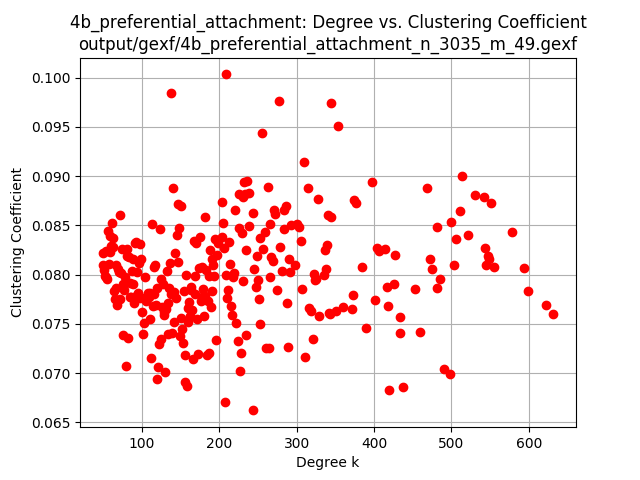
\includegraphics[width=\textwidth]{4b_preferential_attachment_clustering_coeff} % first figure itself
        \caption{Cluster. Coeff}
        \label{fig_4b_preferential_attachment_clustering_coeff}
    \end{minipage}\hfill
    \begin{minipage}{0.5\textwidth}
        \centering
        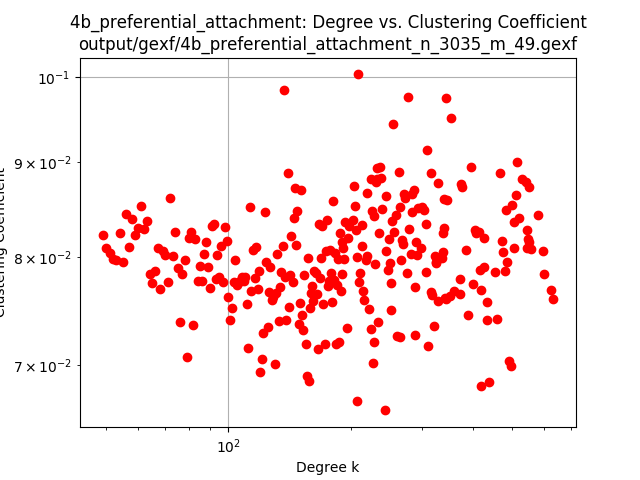
\includegraphics[width=\textwidth]{4b_preferential_attachment_clustering_coeff_log} % second figure itself
        \caption{ Cluster. Coeff in log}
        \label{fig_4b_preferential_attachment_clustering_coeff_log}
    \end{minipage}
\end{figure}


\section{Conclusions and Future Work}

Simple graphical analysis on network is useful for tennis player evaluation.
Both Eigen and Katz centrality gives a good result for player evaluation.
Player network exhibits scale-free model with $\alpha $ approximating 2.1.
To answer question such as which of them is better in serving, returning or win-rate requires further investigation. New rankings can be explored through different match statistics. Constructing & Comparing network for every decade.
%
% ---- Bibliography ----
%
\bibliographystyle{splncs04}
\bibliography{mybib}

All links were last followed on November 21, 2019.

\end{document}
